\question \textbf{HMM profile}

A path of an HMM profile represents an alignment between an input sequence and the profile.

\vspace{0.1 in}

\begin{parts}

%% (a)
  \part Assume Seq1 = ’q1 q2’ and its path is indicated with solid lines. Draw the alignment of Seq1 and the profile.
\begin{figure}[H]
      \centering
      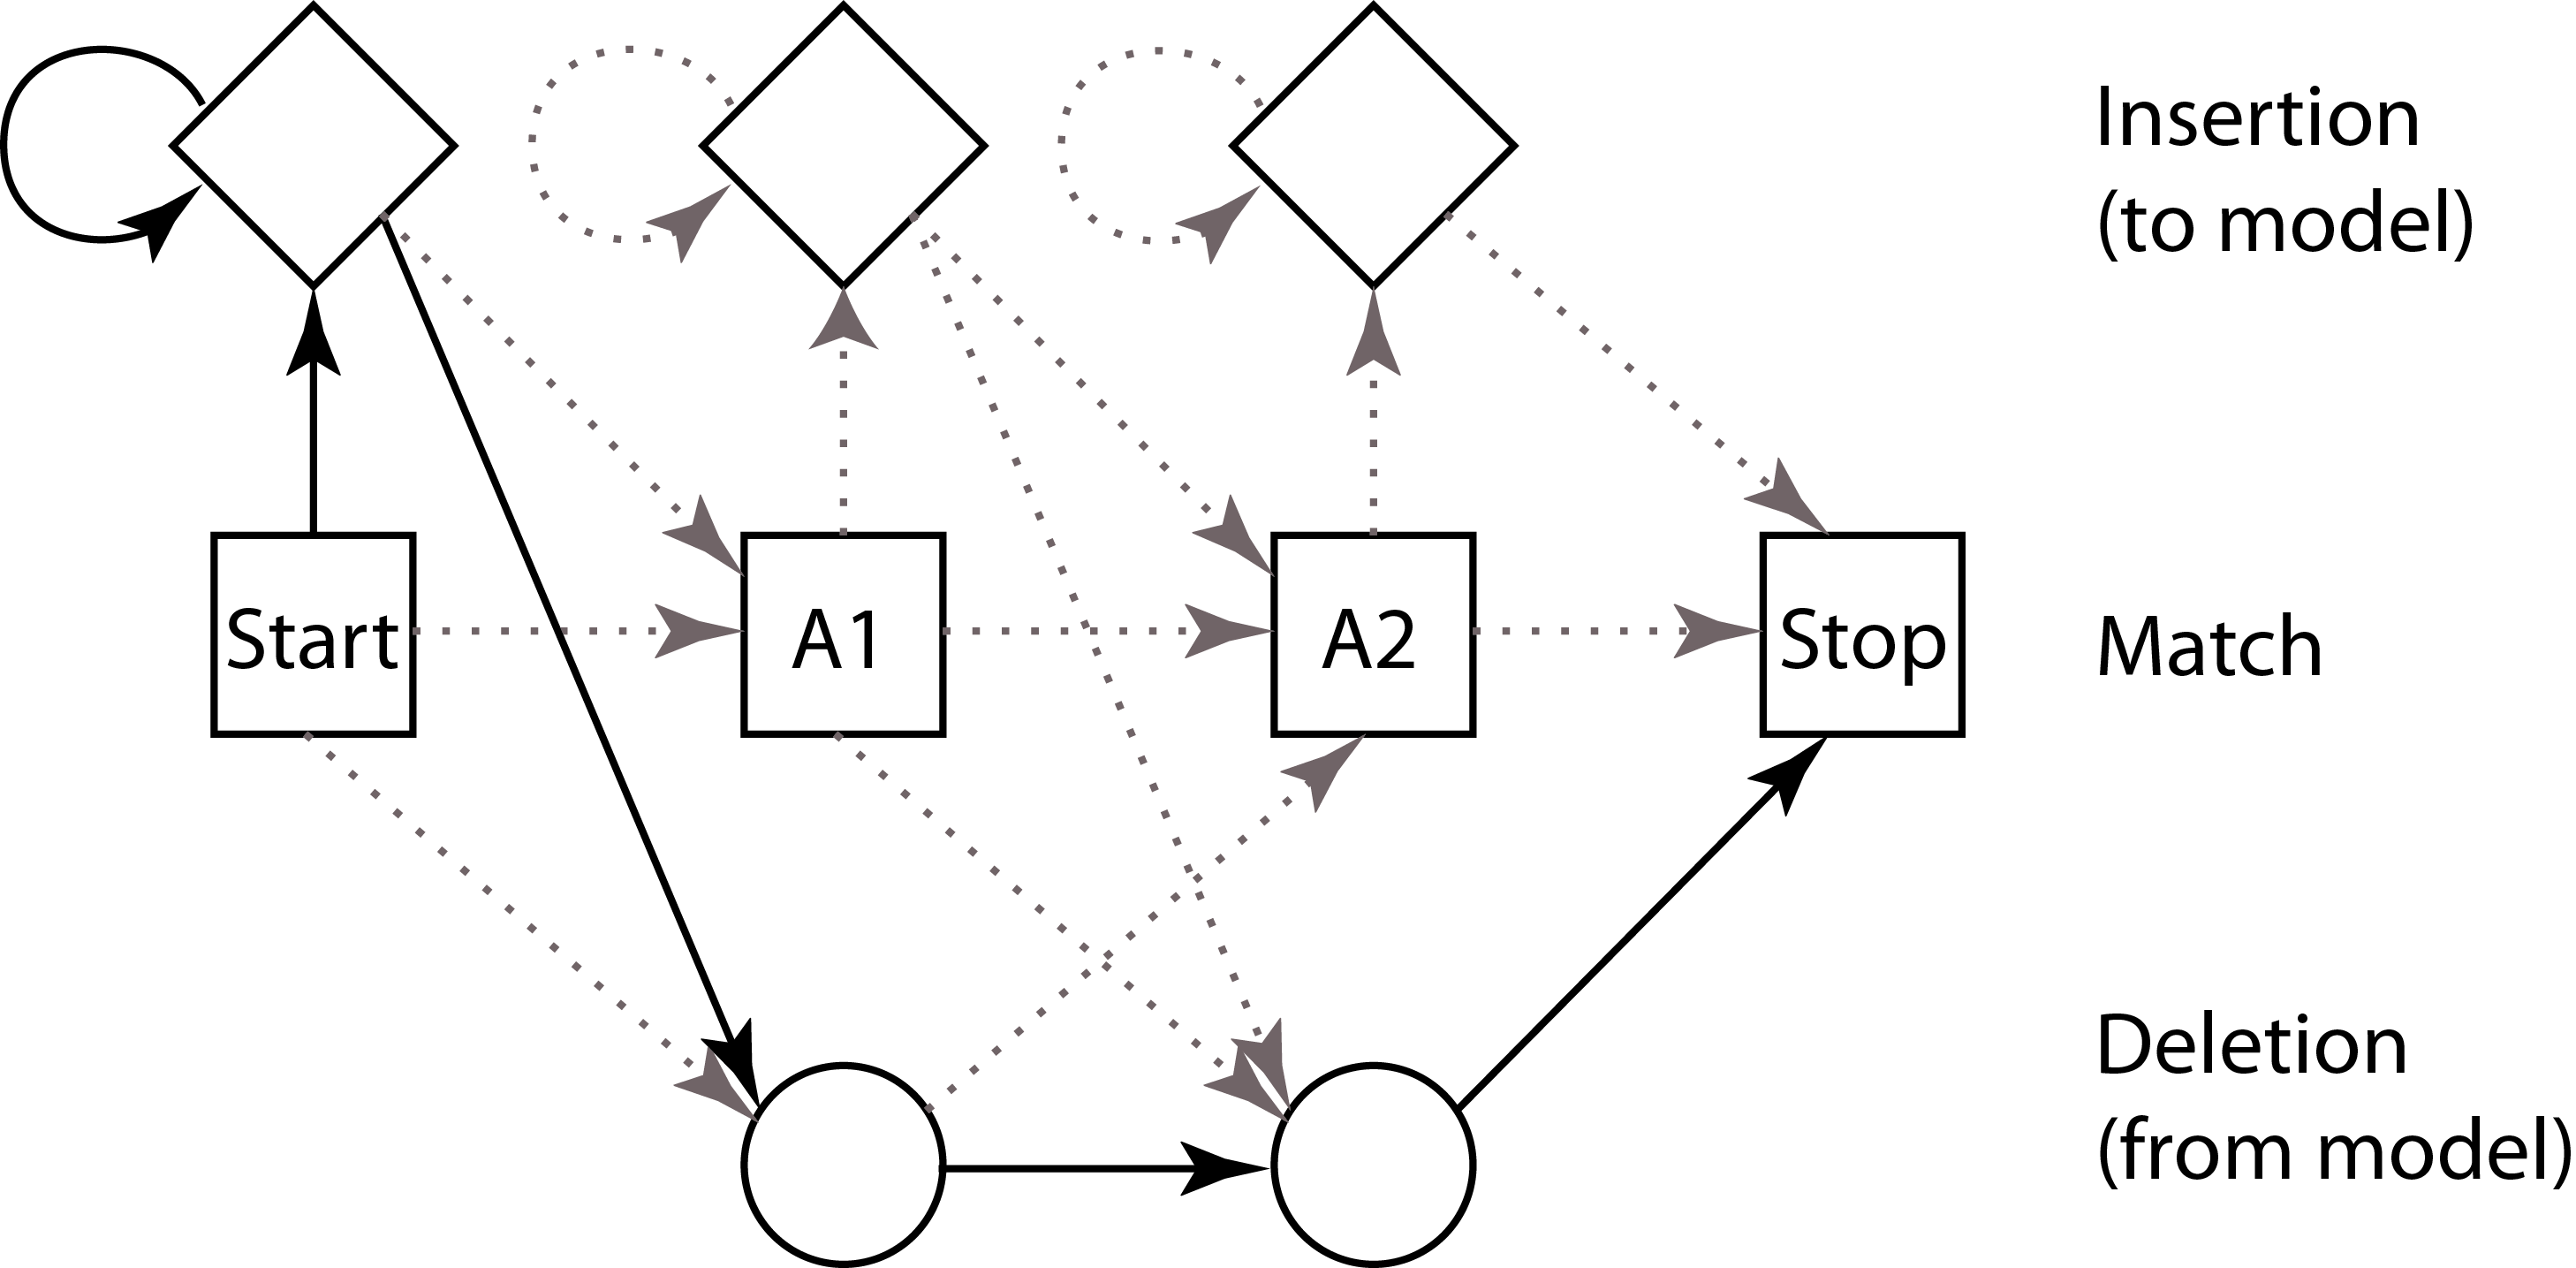
\includegraphics[width=0.6 \textwidth]{fig13/hmm_profile_1.png}
\end{figure}

\begin{solution}[0.7 in]
\begin{verbatim}
   Seq1: q1 q2 -  -
Profile: -  -  A1 A2
\end{verbatim}
\end{solution}

%% (b)
  \part Assume Seq2 = ’q1 q2 q3 q4 q5 q6’ and its path is indicated with solid lines. Draw the alignment of Seq2 and the profile.
\begin{figure}[H]
      \centering
      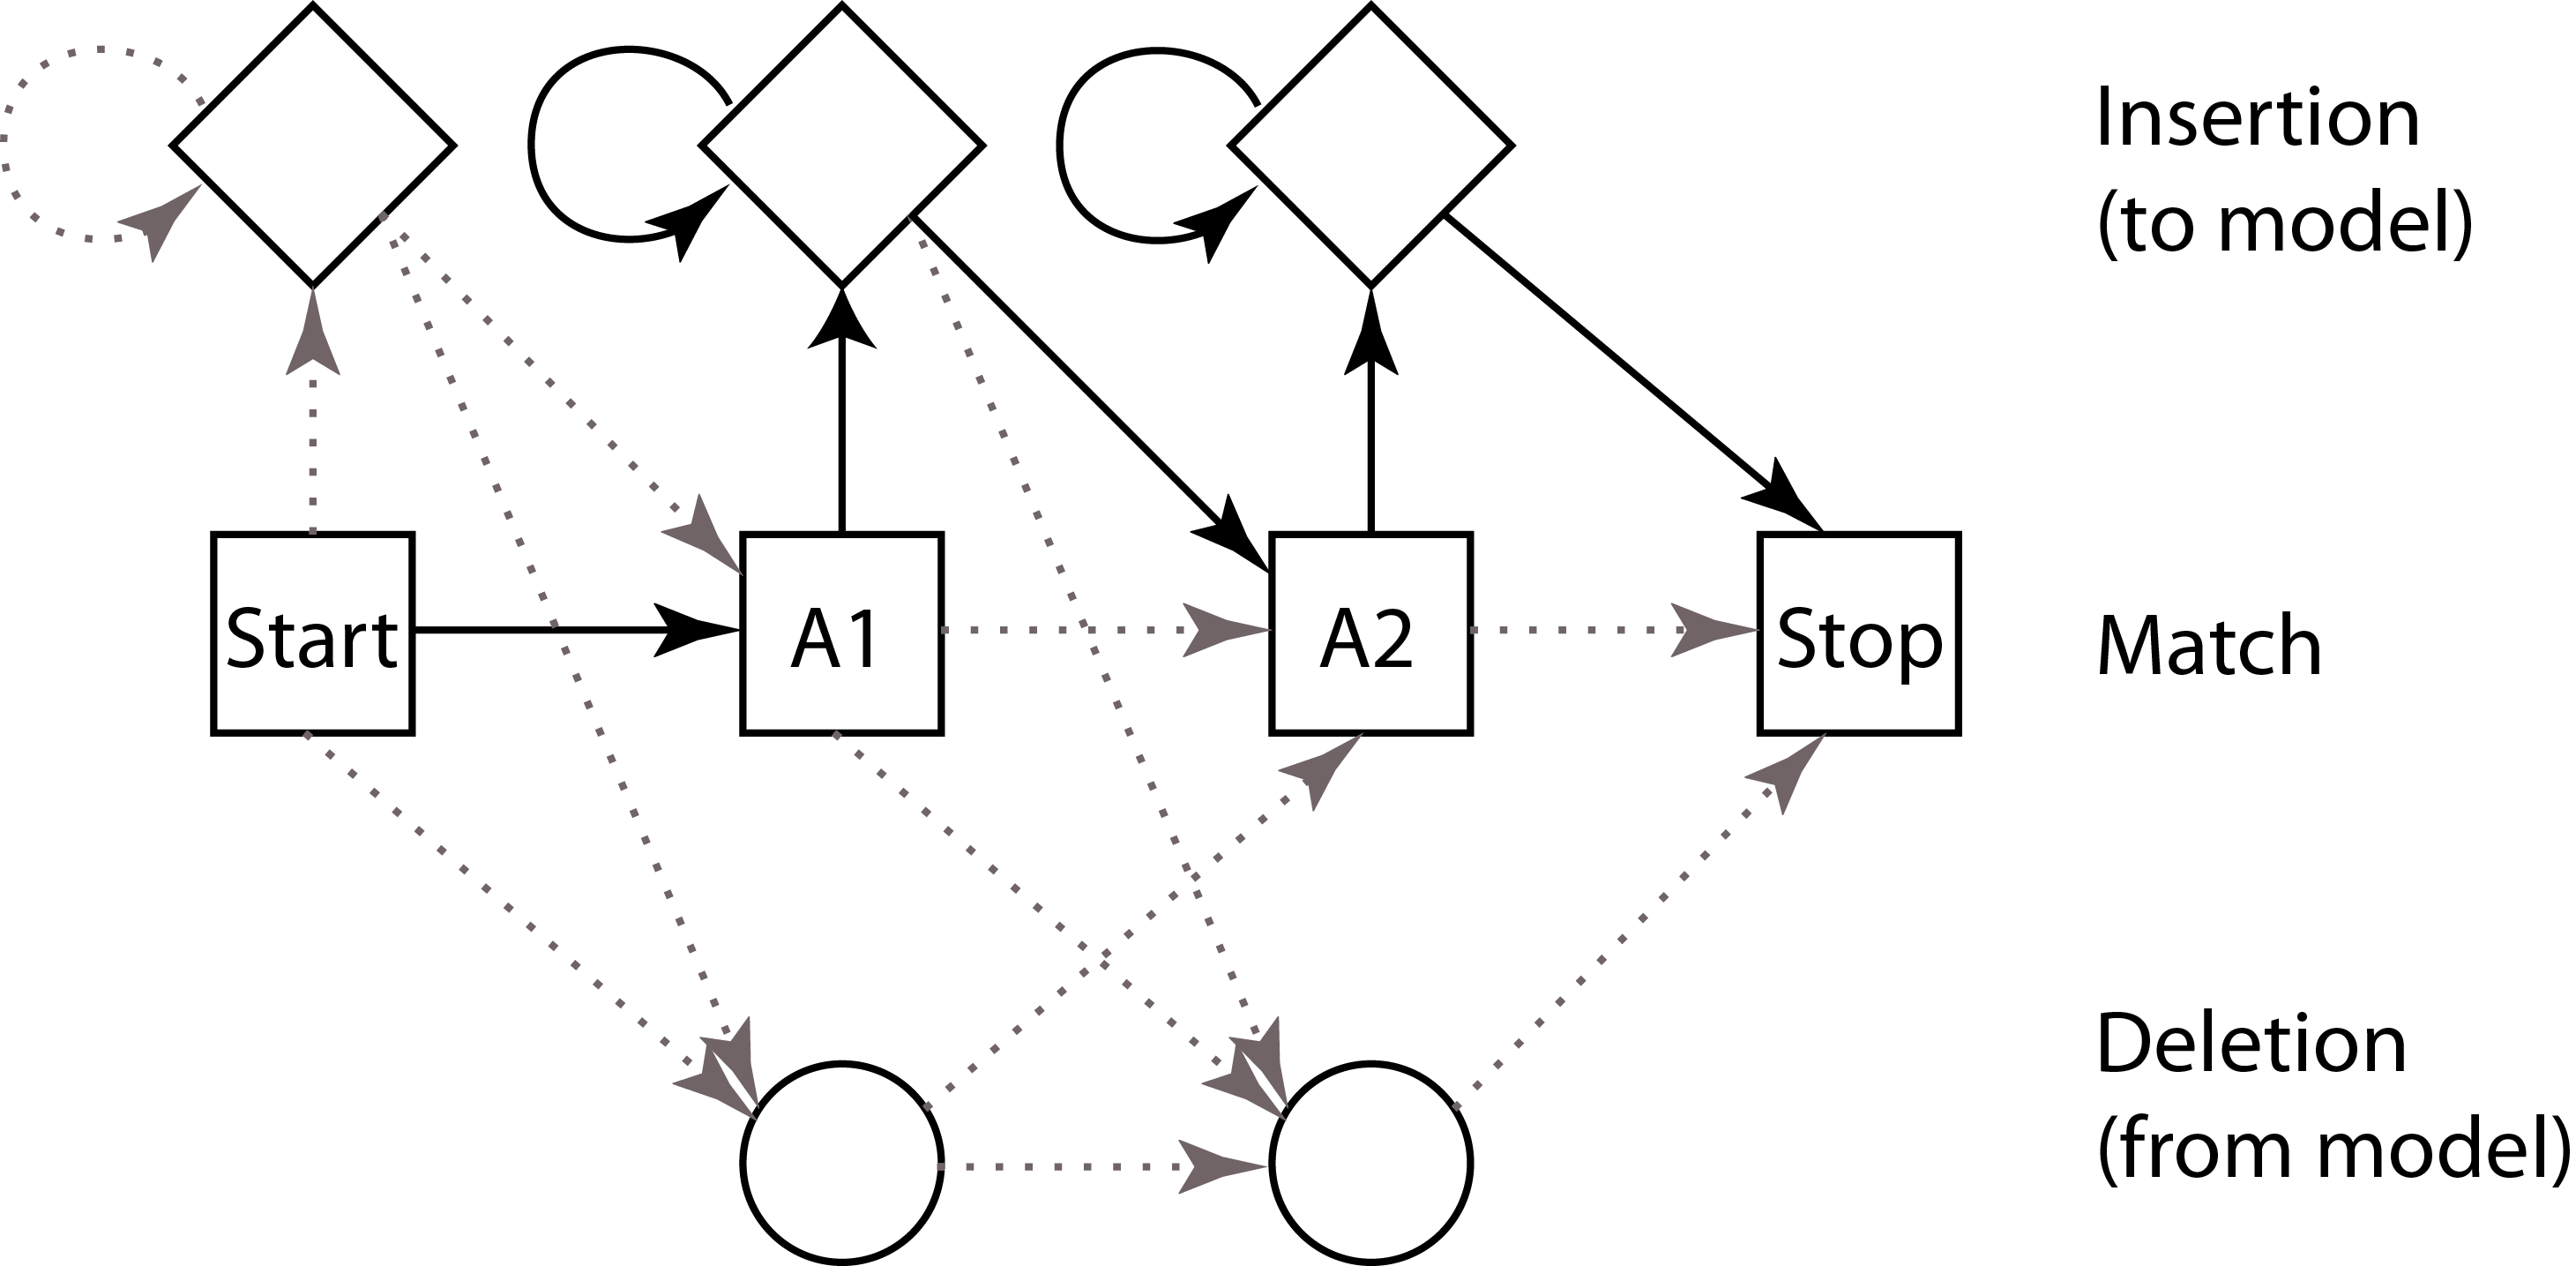
\includegraphics[width=0.6 \textwidth]{fig13/hmm_profile_2.png}
\end{figure}

\begin{solution}[0.7 in]
\begin{verbatim}
   Seq2: q1 q2 q3 q4 q5 q6
Profile: A1 -  -  A2 -  -
\end{verbatim}
\end{solution}

\end{parts}
